\section*{Problema 3}

\textbf{Implemente el algoritmo de cuadratura de Gauss-Legendre y evalua las integrales usando 2, 4 y 10 nodos.}

Se tiene que una manera de aproximar el valor de una integral definida en el intervalo $[-1,1]$ es usando el algoritmo de cuadratura de Gauss-Legendre es:

\begin{equation}
    \int_{-1}^1 f(x) = \sum_i^n \omega_i f(x_i)
\end{equation}

donde $\omega_i,x_i$ es el peso y la raiz i-esima del polinomio de Legendre de grado n respectivamente.

Para una integral definida en el intervalo $[a,b]$ se tiene que la aproximación usando el algoritmo de cuadratura de Gauss-Legendre es:

\begin{equation}
    \int_{a}^b f(x) = \frac{b-a}{2} \sum_i^n \omega_i f\left (\frac{b-a}{2}x_i+\frac{b+a}{2} \right ) \label{eq:problema3}
\end{equation}

\begin{enumerate}
    \item \begin{equation}
              \int_0^\pi xcos(x) dx \label{eq:problema3a}
          \end{equation}

          Usando la aproximación de cuadratuea de Gauss-Legendre (ecuación \ref{eq:problema3}) se obtuvieron los resultados mostrados en la tabla \ref{table:problema3a} y en la figura \ref{fig:problema3a}.

          \begin{table}[H]
              \centering
              \begin{tabular}{ccc} \hline
                  \textbf{Puntos} & \textbf{Resultado} & \textbf{Diferencia} \\ \hline
                  2               & -2.243950          & 0.243950            \\
                  3               & -2.007514          & 0.007514            \\
                  4               & -2.005662          & 0.005662            \\
                  5               & -2.005474          & 0.005474            \\
                  6               & -2.000419          & 0.000419            \\
                  7               & -1.998000          & 0.002000            \\
                  8               & -1.997685          & 0.002315            \\
                  9               & -1.997847          & 0.002153            \\
                  10              & -1.997586          & 0.002414            \\ \hline
              \end{tabular}
              \caption{Resultados y diferencia absoluta del algoritmo de la cuadratura de  Gauss-Legendre para diferentes valores de puntos para la ecuación \ref{eq:problema3a}.}
              \label{table:problema3a}
          \end{table}

          \begin{figure}[H]
              \centering
              \begin{subfigure}[b]{14cm}
                  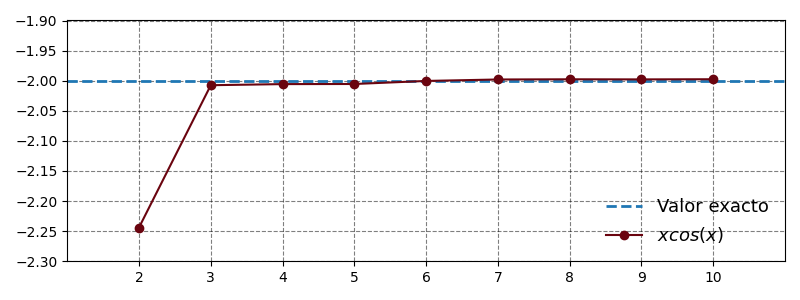
\includegraphics[width=14cm]{Graphics/problema03_fun_f1.png}
                  \caption{Resultados de la integral usando la cuadratura de Gauss-Legendre.}
              \end{subfigure}
              \begin{subfigure}[b]{14cm}
                  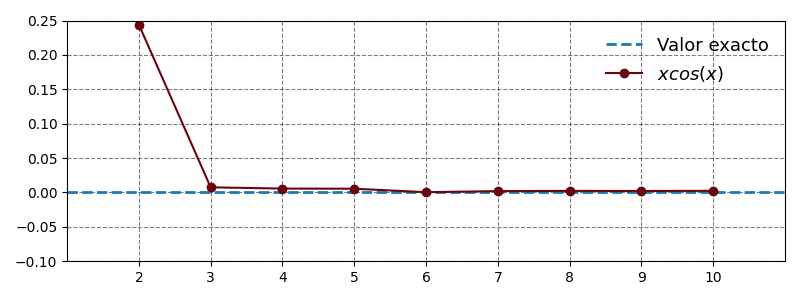
\includegraphics[width=14cm]{Graphics/problema03_diff_f1.png}
                  \caption{Diferencia absoluta entre el algoritmo de Simpson y el valor análitico.}
              \end{subfigure}
              \caption{Resultados usando el algoritmo de cuadratura de Gauss-Legendre con la ecuación \ref{eq:problema3a}.}
              \label{fig:problema3a}
          \end{figure}

    \item \begin{equation}
              \int_{-1}^0 xe^{-x} dx \label{eq:problema3b}
          \end{equation}

          Usando la aproximación de cuadratuea de Gauss-Legendre (ecuación \ref{eq:problema3}) se obtuvieron los resultados mostrados en la tabla \ref{table:problema3b} y en la figura \ref{fig:problema3b}.

          \begin{table}[H]
              \centering
              \begin{tabular}{ccc} \hline
                  \textbf{Puntos} & \textbf{Resultado} & \textbf{Diferencia} \\ \hline
                  2               & -0.998258          & 0.001742            \\
                  3               & -0.988563          & 0.011437            \\
                  4               & -0.999618          & 0.000382            \\
                  5               & -0.990694          & 0.009306            \\
                  6               & -0.998878          & 0.001122            \\
                  7               & -0.994253          & 0.005747            \\
                  8               & -0.998817          & 0.001183            \\
                  9               & -0.995918          & 0.004082            \\
                  10              & -0.998939          & 0.001061            \\ \hline
              \end{tabular}
              \caption{Resultados y diferencia absoluta del algoritmo de la cuadratura de  Gauss-Legendre para diferentes valores de puntos para la ecuación \ref{eq:problema3b}.}
              \label{table:problema3b}
          \end{table}

          \begin{figure}[H]
              \centering
              \begin{subfigure}[b]{14cm}
                  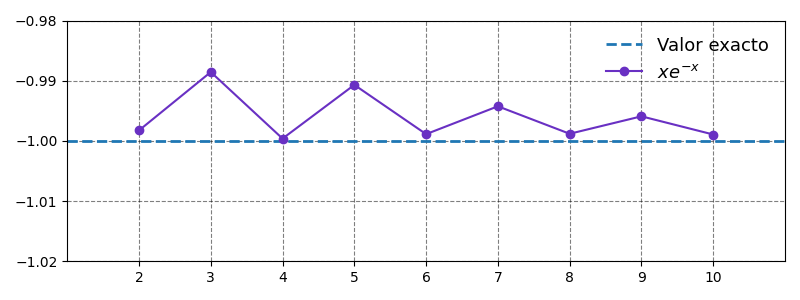
\includegraphics[width=14cm]{Graphics/problema03_fun_f2.png}
                  \caption{Resultados de la integral usando la cuadratura de Gauss-Legendre.}
              \end{subfigure}
              \begin{subfigure}[b]{14cm}
                  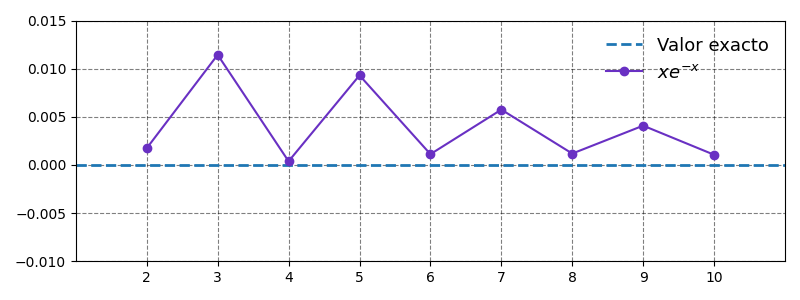
\includegraphics[width=14cm]{Graphics/problema03_diff_f2.png}
                  \caption{Diferencia absoluta entre el algoritmo de Simpson y el valor análitico.}
              \end{subfigure}
              \caption{Resultados usando el algoritmo de cuadratura de Gauss-Legendre con la ecuación \ref{eq:problema3b}.}
              \label{fig:problema3b}
          \end{figure}
\end{enumerate}

En las figuras \ref{fig:problema3a} y \ref{fig:problema3b} se observa que a un número mayor de puntos. Se obtiene una mejor aproximación con un número par de puntos, esto es debido a los pesos del polinomio de Legendre.